\documentclass[a4paper, 11pt]{article}

\usepackage[a4paper,margin=1in]{geometry}
\usepackage[english]{babel}
\usepackage[utf8]{inputenc}
\usepackage[T1]{fontenc}
\usepackage{lmodern}
\usepackage{listings}
\usepackage{graphicx}
\usepackage{amsmath}
\usepackage{framed}
\usepackage{amsfonts}
\usepackage{caption}
\usepackage{subcaption}
\usepackage{listings}
\usepackage{tabularx}
\usepackage{color}
\usepackage[dvipsnames]{xcolor}
\usepackage{fancyhdr}
\usepackage{lastpage}
% \usepackage[round, sort]{natbib}
\usepackage{tikz}

\bibliographystyle {abbrv}
\usetikzlibrary{decorations.pathreplacing, matrix}


\graphicspath{{../imgs/}}


\definecolor{morange}{RGB}{237,106,90}
\definecolor{mgreen}{RGB}{63,127,95}
\definecolor{mpurple}{RGB}{127,0,85}

\lstset{
  basicstyle=\small\ttfamily, % Global Code Style
  captionpos=b, % Position of the Caption (t for top, b for bottom)
  extendedchars=true, % Allows 256 instead of 128 ASCII characters
  tabsize=2, % number of spaces indented when discovering a tab
  columns=fixed, % make all characters equal width
  keepspaces=true, % does not ignore spaces to fit width, convert tabs to spaces
  showstringspaces=false, % lets spaces in strings appear as real spaces
  breaklines=true, % wrap lines if they don't fit
  frame=trbl, % draw a frame at the top, right, left and bottom of the listing
  frameround=tttt, % make the frame round at all four corners
  framesep=4pt, % quarter circle size of the round corners
  numbers=left, % show line numbers at the left
  numberstyle=\tiny\ttfamily, % style of the line numbers
  commentstyle=\color{mgreen}, % style of comments
  keywordstyle=\color{mpurple}, % style of keywords
  stringstyle=\color{morange}, % style of strings
}

% TAILLE DES PAGES (A4 serré)

\setlength{\intextsep}{2em}
\setlength{\parindent}{0pt}
\setlength{\parskip}{1em}
%% \setlength{\textwidth}{17cm}
%% \setlength{\textheight}{24cm}
%% \setlength{\oddsidemargin}{-.7cm}
%% \setlength{\evensidemargin}{-.7cm}
%% \setlength{\topmargin}{-.5in}


\pagestyle{fancy}
\renewcommand{\headrulewidth}{0pt}
\renewcommand{\footrulewidth}{0.6pt}% default is 0pt
\lhead{}
\rhead{}
\lfoot{Page \thepage\ of \pageref{LastPage}}
\rfoot{Rémi Lespinet}
\cfoot{}
\cfoot{}

\newcounter{cquestion}
\renewcommand{\thecquestion}{\arabic{cquestion}}
\newenvironment{question}
{\par \vspace{0.5em} \noindent \stepcounter{cquestion} \hspace{-1em}
 $\bullet$ \underline{Q\thecquestion :}}
{}

\newenvironment{note}
{\begin{framed} \textbf{Note : }}
{\end{framed}}


% Commandes de mise en page
\newcommand{\file}[1]{\lstinline{#1}}
\newcommand{\name}[1]{\emph{#1}}
\newcommand{\Fig}[1]{Fig \ref{#1} p. \pageref{#1}}
\newcommand{\Figure}[1]{Figure \ref{#1} p. \pageref{#1}}
\newcommand{\Tab}[1]{Tab \ref{#1} p. \pageref{#1}}
\newcommand{\Table}[1]{Table \ref{#1} p. \pageref{#1}}
\newcommand{\itemi}{\item[$\bullet$]}
% Commandes color
\newcommand{\colgood}[1]{\color{ForestGreen} #1}
\newcommand{\colbad}[1]{\color{BrickRed} #1}


% Commandes de maths
\newcommand{\function}[3]{#1 : #2 \to #3}
\newcommand{\intn}[2]{\left\{ #1 \dots #2 \right\}}
\newcommand{\intr}[2]{\left[ #1 ; #2 \right]}
\newcommand{\intro}[2]{\left] #1 ; #2 \right[}
\newcommand{\dotp}[2]{\langle #1, #2 \rangle}
\newcommand{\logn}[1]{\ln\left( #1\right)}
%% \newcommand{\det}[1]{\left| #1 \right|}
\newcommand{\pd}[2]{\frac{\partial #1}{\partial #2}}
\newcommand{\norm}[1]{\|#1\|}
\newcommand{\set}[2]{\left\{ #1 \hspace{.5em} ; \hspace{.5em}#2 \right\}}
\newcommand{\tr}[1]{Tr\left( #1 \right)}
\newcommand{\pcond}[2]{p(#1 \hspace{-.2em}\mid\hspace{-.2em} #2)}
\newcommand{\e}[1]{\mathop{\mathbb{E}}\left[#1\right]}


\newcommand{\iid}{i.i.d }
\newcommand{\wrt}{w.r.t }

% Commandes informatique
\newcommand{\pfun}[1]{{\textbf{\texttt{#1}}}}

\newcommand{\ipart}[1]{\vspace{0.5em}\textbf{#1}\vspace{0.5em}}



\pagenumbering{arabic}

\title{\textsc{Reinforcement learning - MVA 2017/2018 \\ \emph{Homework 2}} }
\author{Rémi Lespinet}
\date{}

\begin{document}

\maketitle
\thispagestyle{fancy}

\section{Stochastic Multi-Armed Bandits on Simulated Data}

\subsection{Bernoulli bandit models}

\begin{question}
  % The following section compares the expected regret for the UCB1 and Thomson sampling
  % algorithms for two Benoulli bandit problems with different complexities.
  The figures \ref{fig:ex1-bernoulli-1} and \ref{fig:ex1-bernoulli-2}
  represent two different Bernoulli bandit problems with different
  complexity. For each problem, the left subfigure represents the
  repartition of the arms and the complexity $C(p)$ as defined by the
  \emph{Lai and Robbins} formula \cite{lairobbins85}.  The right
  figure represents the estimation of the expected cumulated regret
  for both algorithm (UCB1 and Thompson Sampling). The value $\rho$
  for UCB1 is equal to $0.5$ for both problems, and the expected
  cumulated regret is computed over $1000$ simulations. Each
  simulation has a horizon $T = 5000$.


  % \begin{table}[h!]
  %   \centering
  %   \begin{tabular}{|c|c|c|c|c|}
  %     \hline
  %     & Arm 0 & Arm 1 & Arm 2 & Arm 3 \\
  %     \hline
  %     $\mu$ & 0.28 & 0.29 & 0.35 & 0.80 \\
  %     \hline
  %   \end{tabular}
  %   \captionof{table}{Parameters for the first Bernoulli bandit} \label{tab:transition-table}
  % \end{table}


  The first chosen problem has 4 arms of means. The
  complexity $C(p) = 2.614$

  The first chosen problem has 5 arms of means $[0.64, 0.18, 0.80, 0.81, 0.29]$ and a
  complexity $C(p) = 34.825$



  % The figure \ref{fig:} represents the first Bernoulli bandit problem. The subfigure
  % \ref{fig:} shows the Bernoulli parameter for each of the $4$ arms with $4$ arms,
  % and a complexity of $C(p) = 0.741$.


  \begin{figure}[ht]
    \centering
    \begin{subfigure}[t]{0.48\textwidth}
      \centering
      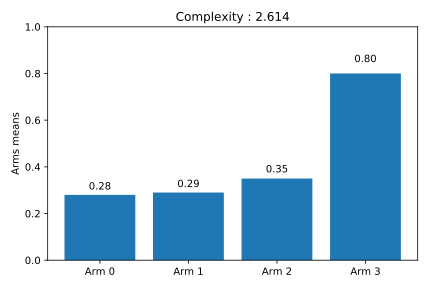
\includegraphics[width=\textwidth]{ex1_bernoulli_arms_1}
      \caption{Representations of the parameters of each arms}\label{fig:ex1-bernoulli-arms-1}
    \end{subfigure}
    \quad
    \begin{subfigure}[t]{0.48\textwidth}
      \centering
      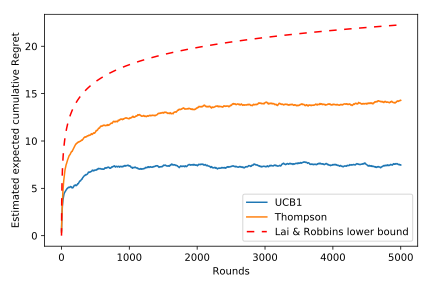
\includegraphics[width=\textwidth]{ex1_bernoulli_regret_1}
      \caption{Estimated expected cumulative regret for UCB1 and TS,
        and Lai-Robbins lower bound}\label{fig:ex1-bernoulli-regret-1}
    \end{subfigure}
    \vskip\baselineskip
    \caption{Representation of the arms means and expected cumulative
      regret for the first chosen Bernoulli bandit}\label{fig:ex1-bernoulli-1}
  \end{figure}

  \begin{figure}[ht]
    \centering
    \begin{subfigure}[t]{0.48\textwidth}
      \centering
      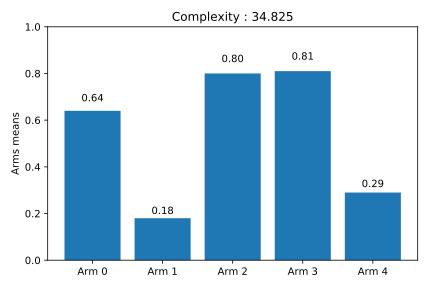
\includegraphics[width=\textwidth]{ex1_bernoulli_arms_2}
      \caption{Representations of the parameters of each arms}\label{fig:ex1-bernoulli-arms-2}
    \end{subfigure}
    \quad
    \begin{subfigure}[t]{0.48\textwidth}
      \centering
      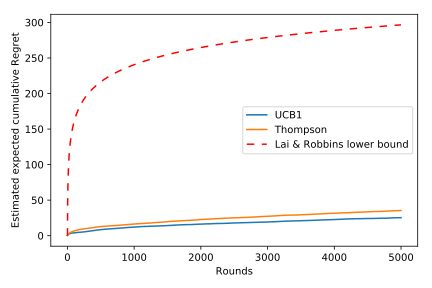
\includegraphics[width=\textwidth]{ex1_bernoulli_regret_2}
      \caption{Estimated expected cumulative regret for UCB1 and TS,
        and Lai-Robbins lower bound}\label{fig:ex1-bernoulli-arms-regret-2}
    \end{subfigure}
    \caption{Representation of the arms means and expected cumulative
      regret for the second chosen Bernoulli bandit}\label{fig:ex1-bernoulli-2}
  \end{figure}

  \newpage
  \ipart{UCB1 vs Thompson}

  In the two presented cases, the estimated expected cumulative regret
  is lower for the UCB1 algorithm than for the Thompson algorithm. But
  we see that this depends on the value of $\rho$ chosen. The figure
  \ref{fig:ex1-ucb1-vs-thompson} presents the results obtained for the
  second Bernoulli bandit problem for two other values of $\rho$.


  \begin{figure}[ht]
    \centering
    \begin{subfigure}[t]{0.48\textwidth}
      \centering
      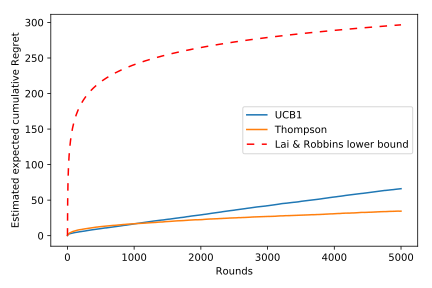
\includegraphics[width=\textwidth]{ex1_bernoulli_regret_2_0_2}
      \caption{$\rho = 0.2$}\label{fig:LDA-A-test}
    \end{subfigure}
    \quad
    \begin{subfigure}[t]{0.48\textwidth}
      \centering
      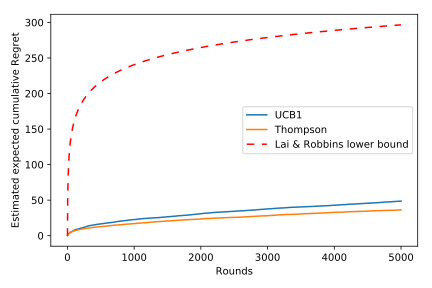
\includegraphics[width=\textwidth]{ex1_bernoulli_regret_2_1_0}
      \caption{$\rho = 1.0$}\label{fig:LDA-A-test}
    \end{subfigure}
    \caption{Comparison of UCB1 and Thompson sampling algorithm for 2
      different values of $\rho$ on the second chosen Bernoulli bandit
      problem}\label{fig:ex1-ucb1-vs-thompson}
  \end{figure}

    % \ipart{Choice of $\rho$}
  This can be explained easily, for the UCB algorithm, we have that By
  Chernoff-Hoeffling
  \begin{equation*}
    P\left(\bar{X} - \e{X} \le \sqrt{\dfrac{\ln{1 / \delta}}{2 n}}\right) \ge 1 - \delta
  \end{equation*}
  If we take $\delta$ such that $\ln{1 / \delta} = \rho^2 \ln{t}$, we have
  \begin{equation*}
    P\left(\bar{X} - \e{X} \le \rho \sqrt{\dfrac{\ln{t}}{2 n}}\right) \ge 1 - \dfrac{1}{t^{\rho^2}}
  \end{equation*}


  \begin{itemize}
  \item If we take $\rho$ too small, the confidence interval length is
    small but we are less confident that $\bar{X} - \e{X}$ lies in
    this interval. Given that the dependency in time is in $\log{t}$,
    this means that if we evaluate a sub-optimal arm as optimal in the
    early iterations of the algorithm, and we discard the optimal one,
    we will end up pulling this sub optimal arm for a very long time
    until the confidence interval eventually grows higher (because of
    the $\log(t)$ term) and we have a chance to correct our mistake,
    and this will have a negative impact on the expected cumulative
    regret.

  \item If we take $\rho$ too large, the confidence intervals for each arm
    will be large, and we will end up exploring a lot more than
    necessary, which also causes the expected cumulative regret to be
    large.
  \end{itemize}

  For a Bernoulli bandit problem with 4 arms (means $0.20$, $0.25$,
  $0.30$, $0.35$), I've run the UCB algorithm 1000 times for different
  values of $\rho$ and a horizon $T = 5000$ and measured the frequency
  of success (that is the best arm being pulled more often than the
  others). The figure \ref{fig:ex1-success-ratio} presents the curve
  obtained.

  \begin{figure}[h]
    \centering
    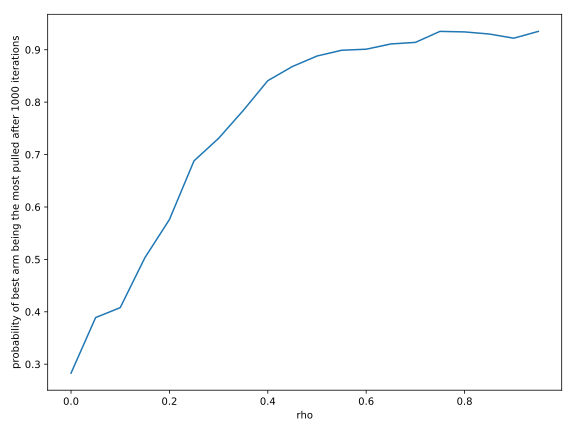
\includegraphics[width=0.6\textwidth]{ex1_success_ratio}
    \caption{Empirical estimation of the probability of the arm with
      maximum mean $mu_{i*}$ being pulled the most as a function of
      $\rho$ for a Bernoulli bandit problem with means ($0.20$,
      $0.25$, $0.30$, $0.35$)}\label{fig:ex1-success-ratio}
  \end{figure}

  \ipart{Advantages of Thompson sampling}

  The main advantages of the Thompson sampling is that it does not
  need a parameter and that the random sampling behavior allow it to
  avoid getting trapped like the UCB1 algorithm due to wrong
  estimations in the early iterations of the algorithm. Another
  advantage is that it provides estimations of the means as a
  continuous probability density function (which allows to compute
  confidence intervals etc ...)

  % \begin{equation*}
  %   \liminf_{T \to \infty}{}
  % \end{equation*}

  \ipart{Intuition of the lower bound}

  Intuitively, when the distributions of each arm are close to each
  other (in the case of a Bernoulli, when the means are close), the
  Kullback-Leibler divergence is close to zero, and hence the
  complexity $C(p)$ is very high, which traduces the fact that it is
  hard to differentiate the arms.
  % \begin{equation*}
  %   KL(x, x + \epsilon) =
  %   - x       \log{\left(1 + \dfrac{\epsilon}{x}    \right)}
  %   - (1 - x) \log{\left(1 - \dfrac{\epsilon}{1 - x}\right)}
  % \end{equation*}

  % \begin{equation*}
  %   KL(x, x + \epsilon) \approx
  %   - x       \left(\dfrac{\epsilon}{x} - \dfrac{\epsilon^2}{2 x^2}    \right)
  %   - (1 - x) \left( - \dfrac{\epsilon}{1 - x} - \dfrac{\epsilon^2}{2(1 - x)^2} \right)
  % \end{equation*}

  % \begin{equation*}
  %   KL(x, x + \epsilon) \approx
  %   \dfrac{\epsilon^2}{2 x} + \dfrac{\epsilon^2}{2(1 - x)}
  % \end{equation*}

\end{question}

\subsection{Non-parametric bandits}

\begin{question}
  First the Thompson sampling algorithm for Bernoulli bandits relies
  on the fact that if the prior distribution of the mean is
  Beta$(\alpha, \beta)$ then the posterior distribution after an
  observation of a Bernoulli sample $x_i$ is also a beta distribution
  Beta$(\alpha + x_i, \beta + (1 - x_i))$
  \begin{equation*}
    \pcond{\mu}{x_i} \propto \pcond{x_i}{\mu} p(\mu) =
    \mu^{x_i} (1 - \mu)^{1 - x_i} \mu^{\alpha - 1} (1 -\mu)^{\beta - 1} = \mu^{\alpha - 1 + x_i} (1 -\mu)^{\beta - x_i}
  \end{equation*}
  In general, when the MAB contains at least an arm that does not
  follow a Bernoulli distribution, because the conjuguate prior
  distribution for such an arm is not the Beta distribution in
  general, we cannot apply the exact same algorithm. The idea
  proposed in \cite{agrawalgoyal12} is to pull the arm, observe the
  reward $\tilde{r}_t$ which is drawn from a probability distribution
  with density $f$ taking values in $[0, 1]$, and then perform a
  Bernoulli trial with probability $\tilde{r}_t$, we note $r_t$ the
  outcome. $r_t$ is a random variable following a Bernoulli
  distribution, and we have
  \begin{equation*}
    p(r_t = 1) = \int_{0}^1 \pcond{r_t = 1}{\tilde{r}_t} f(\tilde{r}_t) d\tilde{r}_t
    = \int_{0}^1 \tilde{r}_t f(\tilde{r}_t) d\tilde{r}_t
    = \e{\tilde{r}_t} = \mu
  \end{equation*}
  Which means that we have constructed a Bernoulli random variable
  with the same mean as the general distribution of the arm and we can
  hence apply the same algorithm using this random variable to update
  the Beta parameters. We can also notice that if an arm follows a
  Bernoulli distribution, the added step has no effect and we then
  recover the Bernoulli Thompson sampling as we can expect.


  We then apply this algorithm as well as UCB1 to a more general
  bandit model where arms are not Bernoulli. The chosen model contains
  4 arms, whose distributions are represented in the figure
  \ref{fig:ex1-bandit-general}.

  \begin{figure}[ht]
    \centering
    \begin{subfigure}[t]{0.50\textwidth}
      \centering
      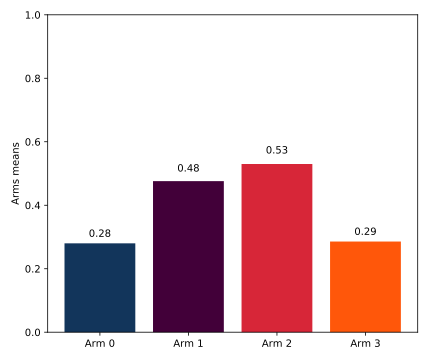
\includegraphics[width=\textwidth]{ex1_general_arms}
      \caption{Representation of the mean of each arm}\label{fig:ex1-bandit-general}
    \end{subfigure}
    \quad
    \begin{subfigure}[t]{0.35\textwidth}
      \centering
      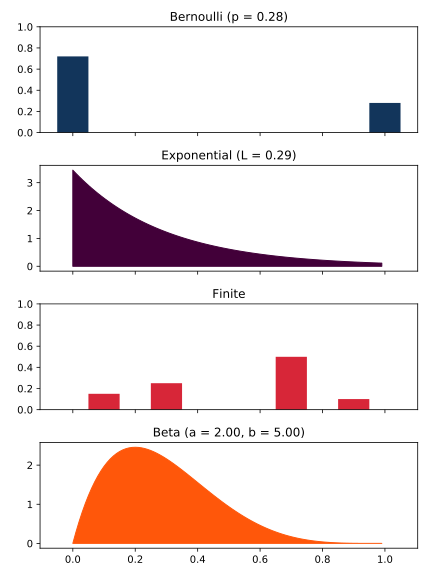
\includegraphics[width=\textwidth]{ex1_general_arms_pdf}
      \caption{Distribution of each arm}\label{fig:ex1-bandit-general-pdf}
    \end{subfigure}
    \caption{Example of a more general bandit model}\label{fig:ex1-bandit-general}
  \end{figure}

  The regret curve for this bandit model is shown in figure
  \ref{fig:ex1-general-regret}.

  The theorem introducing the lower bound \cite{lairobbins85} only
  holds when the distribution of each arms follow the same univariate
  distribution with a single parameter, thus it is not valid for this
  new bandit model. \emph{Burnetas and Katehakis} \cite{burnetas96}
  proved that this bound can be extended to multiparameter or
  nonparametric models. It shows that under mild regularity condition,
  any policy satisfies
  \begin{equation*}
    \liminf_{n \to \infty} \dfrac{R_T}{\log{(T)}} \ge
    \sum_{a: \mu_a < \mu^*} \dfrac{\mu^* - \mu_i}{KL_{\inf}(F_a, \mu^*)}
  \end{equation*}
  with
  \begin{equation*}
    KL_{\inf}(F, \mu) = \inf_{G \in \mathcal{F}: E[G] > \mu} KL(F \| G)
  \end{equation*}
  It is a little more difficult to compute, and hence the figure
  \ref{fig:ex1-general-regret} does not show this lower bound. We can
  still notice that the intuition behind the complexity expression
  remains unchanged, and that this formula is indeed more general than
  the previous one (if we take only arms following Bernoulli
  distributions, we recover the Lai and Robbins lower bound
  expression).

  \begin{figure}[h]
    \centering
    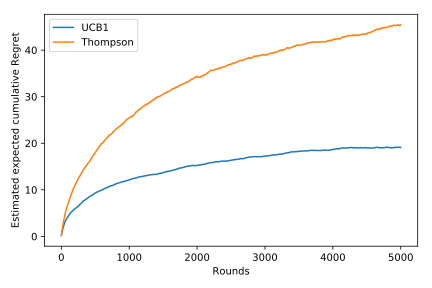
\includegraphics[width=0.6\textwidth]{ex1_general_regret}
    \caption{Estimated expected cumulative regret for UCB1 and TS, and
      Lai-Robbins lower bound}\label{fig:ex1-general-regret}
  \end{figure}


\end{question}


\section{Linear Bandit on Real Data}

\begin{question}
  To write the algorithm efficiently (as suggested in the homework),
  we use the following relations
  \begin{equation*}
    Z_{t+1}^T Z_{t+1} =
    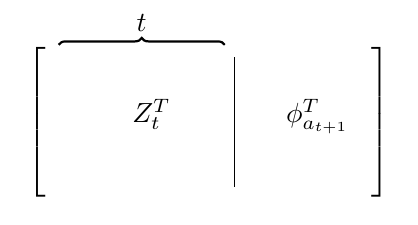
\begin{tikzpicture}[baseline=(current bounding box.center),
      decoration=brace,
      large/.style={font=\large}]
      \matrix (M)[matrix of math nodes, nodes in empty cells,
      left delimiter={[}, right delimiter={]},
      column sep={3em,between origins},
      row sep={2.0em,between origins}
      ]{ &                & & \\
        & Z_t^T          & & \phi_{a_{t+1}}^T\\
        &                & & \\
      };
      \draw(M-1-3.north)--(M-3-3.south);
      % \draw(M-4-1.mid)--(M-4-9.mid);
      % \node[large] at (M-2-7){$0$};
      % \node[large] at (M-7-2){$0$};
      % \node[large] at (M-7-7){$0$};
      % \draw[decorate,transform canvas={xshift=0.3em, yshift=0.8em},thick] (M-1-1.mid west) -- node[above=2pt]{$n$}(M-1-3.mid east);
      \draw[decorate,transform canvas={yshift=0.8em},thick] (M-1-1.west) -- node[above=1pt]{$t$}(M-1-3.west);
      % \draw[decorate,transform canvas={xshift=2.2em},thick] (M-7-5.north) -- node[right=1pt]{$n$}(M-11-5.south);
      % \draw[decorate,thick] (M-9-9.north) -- node[below=2pt]{$n$}(M-9-5.north);
    \end{tikzpicture}
    \cdot
    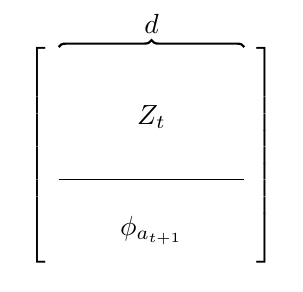
\begin{tikzpicture}[baseline=(current bounding box.center),
      decoration=brace,
      large/.style={font=\large}]
      \matrix (M)[matrix of math nodes, nodes in empty cells,
      left delimiter={[}, right delimiter={]},
      column sep={3.0em,between origins},
      row sep={2.0em,between origins}
      ]{ &                & \\
        & Z_t            & \\
        &                & \\
        & \phi_{a_{t+1}} & \\
      };
      \draw(M-3-1.west)--(M-3-3.east);
      % \draw(M-4-1.mid)--(M-4-9.mid);
      % \node[large] at (M-2-7){$0$};
      % \node[large] at (M-7-2){$0$};
      % \node[large] at (M-7-7){$0$};
      % \draw[decorate,transform canvas={xshift=0.3em, yshift=0.8em},thick] (M-1-1.mid west) -- node[above=2pt]{$n$}(M-1-3.mid east);
      \draw[decorate,transform canvas={yshift=0.8em},thick] (M-1-1.west) -- node[above=1pt]{$d$}(M-1-3.east);
      % \draw[decorate,transform canvas={xshift=2.2em},thick] (M-7-5.north) -- node[right=1pt]{$n$}(M-11-5.south);
      % \draw[decorate,thick] (M-9-9.north) -- node[below=2pt]{$n$}(M-9-5.north);
    \end{tikzpicture}
    = Z_t^T Z_t + \phi_{a_{t+1}}^T \phi_{a_{t+1}}
  \end{equation*}
  and
  \begin{equation*}
    Z_{t+1}^T y_{t+1} =
    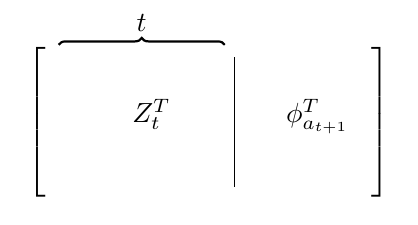
\begin{tikzpicture}[baseline=(current bounding box.center),
      decoration=brace,
      large/.style={font=\large}]
      \matrix (M)[matrix of math nodes, nodes in empty cells,
      left delimiter={[}, right delimiter={]},
      column sep={3em,between origins},
      row sep={2.0em,between origins}
      ]{ &                & & \\
        & Z_t^T          & & \phi_{a_{t+1}}^T\\
        &                & & \\
      };
      \draw(M-1-3.north)--(M-3-3.south);
      % \draw(M-4-1.mid)--(M-4-9.mid);
      % \node[large] at (M-2-7){$0$};
      % \node[large] at (M-7-2){$0$};
      % \node[large] at (M-7-7){$0$};
      % \draw[decorate,transform canvas={xshift=0.3em, yshift=0.8em},thick] (M-1-1.mid west) -- node[above=2pt]{$n$}(M-1-3.mid east);
      \draw[decorate,transform canvas={yshift=0.8em},thick] (M-1-1.west) -- node[above=1pt]{$t$}(M-1-3.west);
      % \draw[decorate,transform canvas={xshift=2.2em},thick] (M-7-5.north) -- node[right=1pt]{$n$}(M-11-5.south);
      % \draw[decorate,thick] (M-9-9.north) -- node[below=2pt]{$n$}(M-9-5.north);
    \end{tikzpicture}
    \cdot
    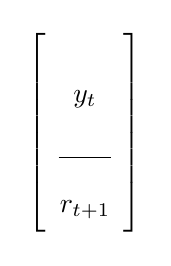
\begin{tikzpicture}[baseline=(current bounding box.center),
      decoration=brace,
      large/.style={font=\large}]
      \matrix (M)[matrix of math nodes, nodes in empty cells,
      left delimiter={[}, right delimiter={]},
      column sep={0.6em,between origins},
      row sep={2.0em,between origins}
      ]{ &         & \\
        & y_t     & \\
        &         & \\
        & r_{t+1} & \\
      };
      \draw(M-3-1.west)--(M-3-3.east);
      % \draw(M-4-1.mid)--(M-4-9.mid);
      % \node[large] at (M-2-7){$0$};
      % \node[large] at (M-7-2){$0$};
      % \node[large] at (M-7-7){$0$};
      % \draw[decorate,transform canvas={xshift=0.3em, yshift=0.8em},thick] (M-1-1.mid west) -- node[above=2pt]{$n$}(M-1-3.mid east);
      % \draw[decorate,transform canvas={yshift=0.8em},thick] (M-1-1.west) -- node[above=1pt]{$d$}(M-1-3.east);
      % \draw[decorate,transform canvas={xshift=2.2em},thick] (M-7-5.north) -- node[right=1pt]{$n$}(M-11-5.south);
      % \draw[decorate,thick] (M-9-9.north) -- node[below=2pt]{$n$}(M-9-5.north);
    \end{tikzpicture}
    = Z_t^T y_t + r_{t + 1} \phi_{a_{t+1}}^T
  \end{equation*}
  Hence, if we note
  \begin{equation*}
    W_{t + 1} = Z_{t+1}^T Z_{t+1} + \lambda I_{d}
  \end{equation*}
  and
  \begin{equation*}
    V_{t + 1} = Z_{t+1}^T y_{t+1}
  \end{equation*}
  We have the update formulas
  \begin{framed}
    \begin{equation*}
      \begin{array}{ll}
        W_{t + 1} &= W_t + \phi_{a_{t+1}}^T \phi_{a_{t+1}} \\[0.6em]
        V_{t + 1} &= V_t + r_{t+1} \phi_{a_{t+1}}^T \\
      \end{array}
    \end{equation*}
  \end{framed}
\end{question}

The figure \ref{fig:ex2-comp-regret} compares the performances of
linUCB against the two following algorithm (in term of estimated
expected regret)
\begin{itemize}
\item Random policy : (Pure exploration) Take a random arm (propose a
  random movie) uniformly at each iteration
\item Epsilon greedy policy : Initialize by taking all arms, explore
  with probability $\epsilon$ and exploit with probability
  $1 - \epsilon$
\end{itemize}
Notice that these two algorithms do not use the context.

I could have also compared the evolution of the estimated distance to
the real theta for each algorithm, in fact, we can computed an
$\hat{\theta}_t$ for the epsilon greedy algorithm from the equality
\begin{equation*}
  \hat{r}_t(a) = \phi_a^T \hat{\theta}_t
\end{equation*}
by computing the pseudo-inverse of $\phi_a^T$ and right multiply this
matrix by our current estimate of the rewards. But since the Epsilon
Greedy algorithm starts by taking all arms ($207$), it already has a
good estimate of $\theta^*$ before actually starting the greedy
strategy.

\begin{figure}[h]
  \centering
  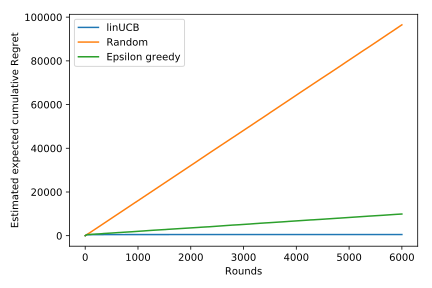
\includegraphics[width=0.55\textwidth]{ex2_comp_regret}
  \caption{Comparison of the estimated expected regret for the
    different algorithm implemented (regularization parameter $\lambda = 0.1$)}\label{fig:ex2-comp-regret}
\end{figure}

\ipart{Performances of linUCB}

We see that the linUCB algorithm is very effective, experimentally for
a value of $\alpha = 1.0$, over $100$ run, the algorithm found the
best arm $100\%$ of the time and started to exploit it after about
$12$ draws in average. This would of course be impossible if we would
not use the context (there are $207$ arms, so this is impossible to
pretend to know the optimal arm if we don't at least pull one time
each arm).

\newpage
\ipart{Trying different values of $\alpha$}

The figure \ref{fig:ex2-linUCB-alpha} shows the impact of $\alpha$ on
the estimated expected regret and on the distance
$\norm{\theta_t - \theta^*}$ between the estimate of $\theta_t$ and
the real value $\theta^*$ (provided)

As expected, as $\alpha$ increases, we give more importance to arms
which are the most incertain (and less importance to the information
we gain on the rewards of the arms), this means we explore more and
we exploit less. In the figure \ref{fig:ex2-linUCB-alpha}, the
consequences are that the regret is higher (we exploit more), and the
aveage distance to the real theta decreases (we gain information about
the distributions of the arms).

As in the UCB1 case, if we take a very small value of $\alpha$, the
algorithm will try to estimate the value of $\theta^*$ with a very
small number of draws, and might then conclude about the optimality of
a sub-optimal arm, which it will then pull for the rest of the
simulation. For example if $\alpha=0.3$, we see that the algorithm
draws in average $3$ arms before concluding about the optimality of an
arm and then pull it to the end of time. This explains the observed
behavior in the figure \ref{fig:ex2-linUCB-alpha-regret} for
$\alpha = 0.3$ (the algorithm pulls the same sub-optimal arm after the
third iteration, which induces a regret at each iteration).

\begin{figure}[ht]
  \centering
  \begin{subfigure}[t]{0.48\textwidth}
    \centering
    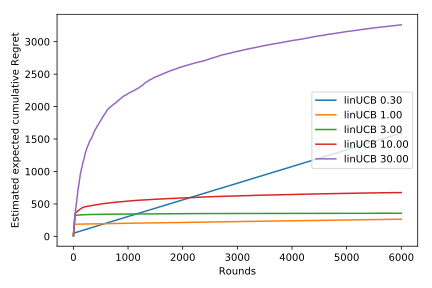
\includegraphics[width=\textwidth]{ex2_linUCB_alpha_regret}
    \caption{Impact on the regret}\label{fig:ex2-linUCB-alpha-regret}
  \end{subfigure}
  \quad
  \begin{subfigure}[t]{0.48\textwidth}
    \centering
    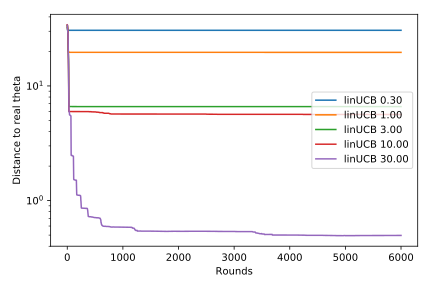
\includegraphics[width=\textwidth]{ex2_linUCB_alpha_dist}
    \caption{Impact on $\norm{\theta_t - \theta^*}$}\label{fig:ex2-linUCB-alpha-dist}
  \end{subfigure}
  \caption{Impact of $\alpha$ on the regret and the distance to the
    real theta (average over 20 simulations of horizon $T=6000$ with
    $\lambda=0.1$)}\label{fig:ex2-linUCB-alpha}
\end{figure}


\newpage
\bibliography{references}


\end{document}

%% \begin{figure}[p]
%%   \centering
%%   \begin{subfigure}[t]{0.40\textwidth}
%%     \centering
%%     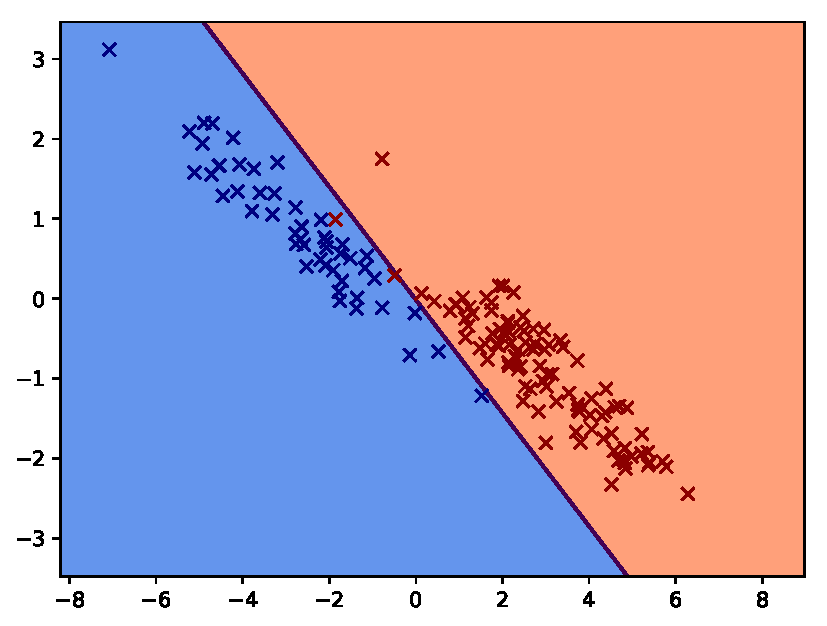
\includegraphics[width=\textwidth]{LDA_classificationA_train}
%%     \caption{Training observations A ($150$ points)}\label{fig:LDA-A-train}
%%   \end{subfigure}
%%   \quad
%%   \begin{subfigure}[t]{0.40\textwidth}
%%     \centering
%%     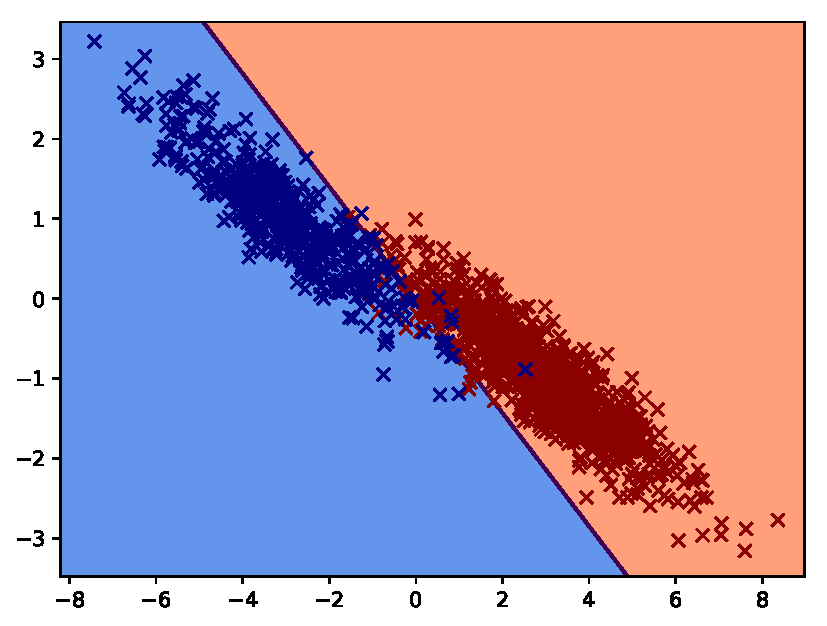
\includegraphics[width=\textwidth]{LDA_classificationA_test}
%%     \caption{Test observations A ($1500$ points)}\label{fig:LDA-A-test}
%%   \end{subfigure}
%%   \vskip\baselineskip
%%   \begin{subfigure}[t]{0.40\textwidth}
%%     \centering
%%     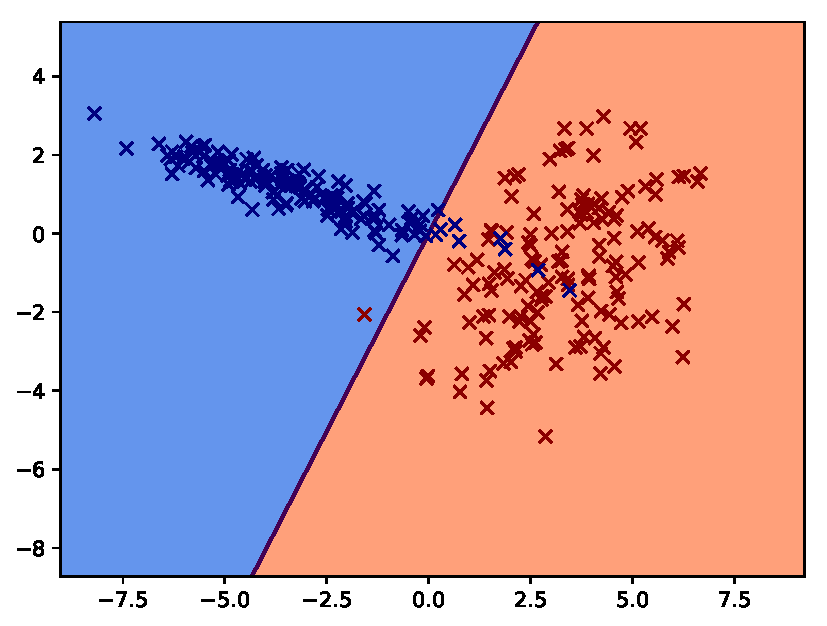
\includegraphics[width=\textwidth]{LDA_classificationB_train}
%%     \caption{Training observations B ($150$ points)}\label{fig:LDA-B-train}
%%   \end{subfigure}
%%   \quad
%%   \begin{subfigure}[t]{0.40\textwidth}
%%     \centering
%%     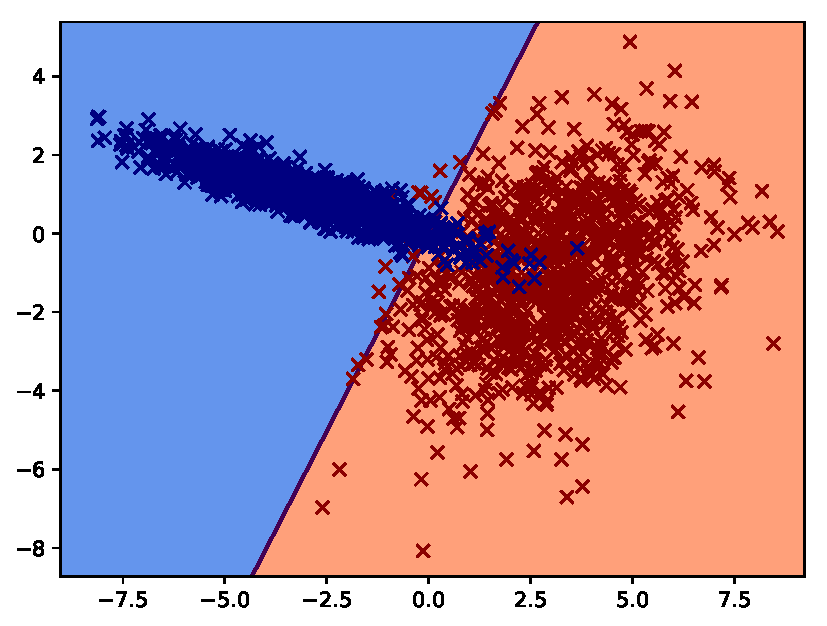
\includegraphics[width=\textwidth]{LDA_classificationB_test}
%%     \caption{Test observations B ($1500$ points)}\label{fig:LDA-B-test}
%%   \end{subfigure}
%%   \vskip\baselineskip
%%   \begin{subfigure}[t]{0.40\textwidth}
%%     \centering
%%     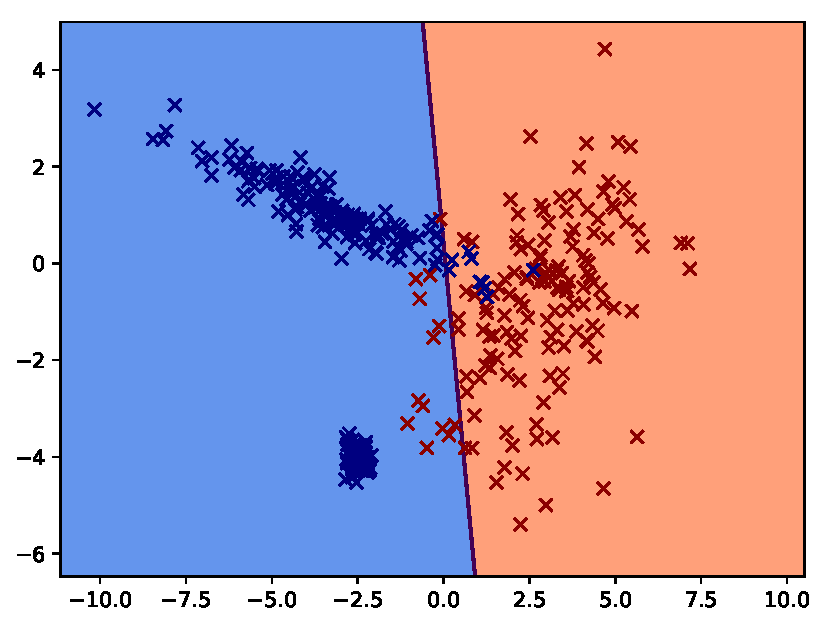
\includegraphics[width=\textwidth]{LDA_classificationC_train}
%%     \caption{Training observations C ($150$ points)}\label{fig:LDA-C-train}
%%   \end{subfigure}
%%   \quad
%%   \begin{subfigure}[t]{0.40\textwidth}
%%     \centering
%%     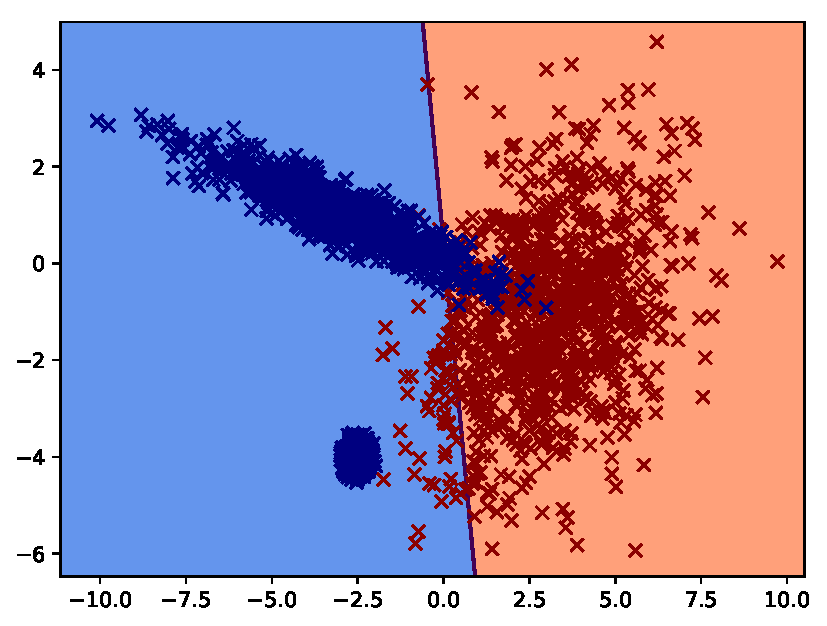
\includegraphics[width=\textwidth]{LDA_classificationC_test}
%%     \caption{Test observations C ($1500$ points)}\label{fig:LDA-C-test}
%%   \end{subfigure}
%%   \caption{Sample data and decision boundary representation for the LDA classifier on the three files}\label{fig:LDA}
%% \end{figure}




  % \begin{table}[h!]
  %   \centering
  %   \begin{tabular}{|c|c|c|c||c|c|c|}
  %     \hline
  %     & \multicolumn{3}{c||}{\textbf{a0}} & \multicolumn{3}{c|}{\textbf{a1}}\\
  %     \hline
  %     & s0 & s1 & s2 & s0 & s1 & s2 \\
  %     \hline
  %     s0 & 0.45 & 0.00 & 0.55 & 0.00 & 0.00 & 1.00 \\
  %     s1 & 0.00 & 0.00 & 1.00 & 0.50 & 0.40 & 0.10 \\
  %     s2 & 0.60 & 0.00 & 0.40 & 0.00 & 0.90 & 0.10 \\
  %     \hline
  %   \end{tabular}
  %   \captionof{table}{Representation of the transition table
  %     corresponding to the graph} \label{tab:transition-table}
  % \end{table}

  % \begin{figure}[h]
  %   \centering
  %   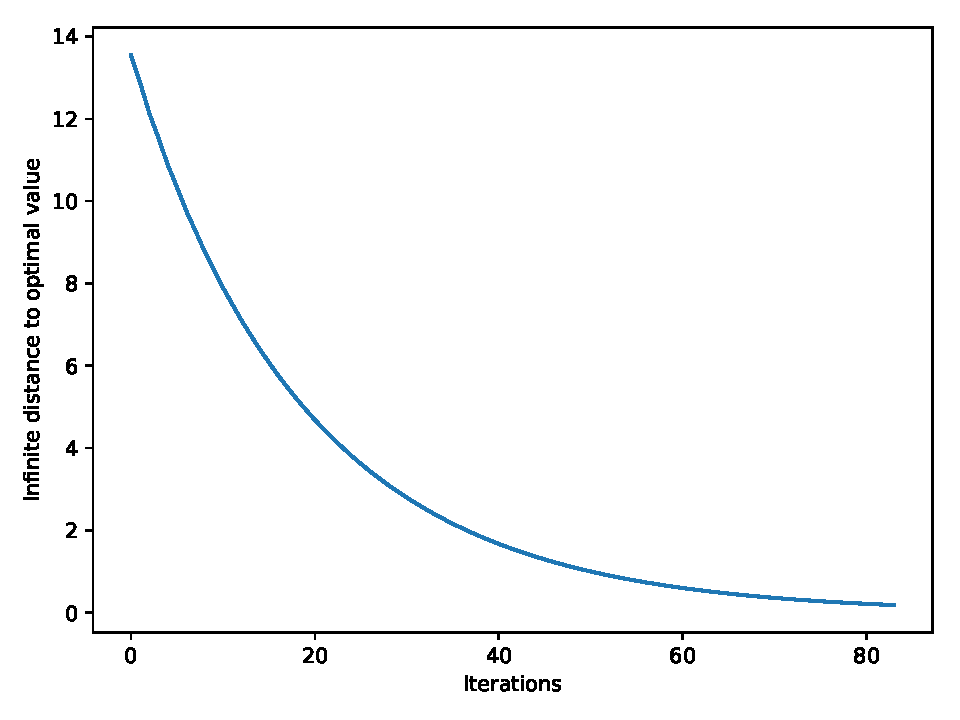
\includegraphics[width=0.7\textwidth]{VI_convergence}
  %   \caption{Convergence of the value iteration algorithm}\label{fig:VI-convergence}
  % \end{figure}
